\section{Introduction}\label{sec:intro}

Population health research is becoming increasingly based on data-driven methods
(as opposed to those designed solely by clinical experts) for patient-centred
care through the advent of accessible software and a relative abundance of
electronic data. A vital part of such research is to better understand the
healthcare needs and behaviours of a population, and it can be beneficial to
find an appropriate segmentation of that population; such a segmentation allows
for finer-grained analysis of groups in the population that share some form of
homogeneity. One commonly used method for such patient-centred analysis is that
of patient flow and their interaction with the healthcare system.

However, this process relies heavily on detailed data --- about both the system
and the population within that system --- which may limit research where
sophisticated data pipelines are not yet in place. This work demonstrates how
this issue may be overcome using administrative, spell-level, hospital data,
i.e.\ a dataset that summarises patient spells. This data is then used to build
a patient clustering that feeds into a multi-class queuing model. Specifically,
this work examines records of patient spells from the National Health Service
(NHS) Wales Cwm Taf Morgannwg University Health Board (UHB) that present chronic
obstructive pulmonary disease (COPD).  COPD is of particular interest to Cwm Taf
Morgannwg UHB as the condition is known to often present as a comorbidity in
patients~\cite{Houben2019} and it was found that they had the highest prevalence
of the condition across all the Welsh health boards in an internal report by NHS
Wales.

% TODO No reference for graph sent by Kendal but is this alright?

% TODO Image of process: administrative data -> extract service parameters ->
%                        validate parameters with Wasserstein distance ->
%                        continue with queuing model as normal

The remainder of the paper is structured as follows: Section~\ref{sec:intro}
provides a literature review, and an overview of the data and its clustering;
Section~\ref{sec:model} describes the queuing model used and the estimation of
its parameters; Section~\ref{sec:scenarios} presents a number of what-if
scenarios with insight provided by the model parameterisation and the
clustering; Section~\ref{sec:conclusion} concludes the paper. Although the data
is confidential and may not be published, the source code used in this paper is
available online at~\url{https://github.com/daffidwilde/copd-paper}.

\subsection{Literature review}\label{subsec:review}

Given the subject matter of this work, the relevant literature spans much of
operational research in healthcare and the focus of this review is on the
principal topics of segmentation analysis, queuing models applied to hospital
systems, and the handling of missing or incomplete data for such queues.

\subsubsection{Segmentation analysis}

Segmentation analysis allows for the targeted analysis of otherwise
heterogeneous datasets and encompasses several techniques from operational
research, statistics and machine learning. One of the most desirable qualities
of this kind of analysis is the ability to glean and communicate simplified
summaries of patient needs to stakeholders within a healthcare
system~\cite{Vuik2016b, Yoon2020}. For instance, clinical profiling often
forms part of the wider analysis where each segment can be summarised in a
phrase or infographic~\cite{Vuik2016a, Yan2019}.

The review for this work identified three commonplace groups of patient
characteristics used to segment a patient population: their system
utilisation metrics, their clinical attributes and their pathway. The latter
is not used to segment the patients directly but rather groups their movements
through a healthcare system. This is typically done via process
mining.~\cite{Arnolds2018}~and~\cite{Delias2015} demonstrate how this technique
can be used to improve the efficiency of a hospital system as opposed to
tackling the more relevant issue of patient-centred care. The remaining
characteristics can be segmented with a number of techniques but recent works
tend to use unsupervised methods, typically latent class analysis (LCA) or
clustering~\cite{Yan2018}.

LCA is a statistical, model-based method used to identify groups (called latent
classes) in data by relating its observations to some unobserved (latent),
categorical attribute. This attribute has multiple categories, each
corresponding to a latent class. The discovered relations are then used to
separate the observations into latent classes according to their maximum
likelihood class membership~\cite{Hagenaars2002,Lazarsfeld1968}. This method has
proved useful in the study of comorbidity patterns as
in~\cite{Kuwornu2014,Larsen2017} where combinations of demographic and clinical
attributes are related to various subgroups of chronic diseases.

Similarly to LCA, clustering identifies groups (clusters) in data to produce a
labelling of its instances. However, clustering includes a wide variety of
methods where the common theme is to maximise homogeneity within, and
heterogeneity between, each cluster~\cite{Everitt2011}. The \(k\)-means paradigm
is the most popular form of clustering in literature. The method iteratively
partitions numerical data into \(k \in \mathbb{N}\) distinct parts where \(k\)
is fixed a priori. This method has proved popular as it is easily scalable and
its implementations are concise~\cite{Olafsson2008,Wu2009}. In addition to
\(k\)-means, hierarchical clustering methods can be effective if a suitable
number of parts cannot be found initially~\cite{Vuik2016a}. Although, supervised
hierarchical segmentation methods such as classification and regression trees
(as in~\cite{Harper2006}) have been used where an existing, well-defined label
is of particular significance.

\subsubsection{Queuing models}

Since the seminal works by Erlang~\cite{Erlang1917,Erlang1920} established
the core concepts of queuing theory, the application of queues and queuing
networks to real services has become abundant including the healthcare service.
By applying these models to healthcare settings, many aspects of the underlying
system can be studied. A common area of study in healthcare settings is of
service capacity.~\cite{McClain1976} is an early example of such work where
acute bed capacity was determined using hospital occupancy data. Meanwhile, more
modern works such as~\cite{Palvannan2012,Pinto2014} consider wider sources of
data (where available) to build their queuing models. Moreover, the output of
a model is catered more towards being actionable --- as is the prerogative of
operational research. For instance,~\cite{Pinto2014} devises new categorisations
for both hospital beds and arrivals that are informed by the queuing model.
A further example is~\cite{Komashie2015} where queuing models are used to
measure and understand satisfaction amongst patients and staff.

In addition to these theoretic models, healthcare queuing research has expanded
to include computer simulation models. The simulation of queues, or networks
thereof, have the benefit of being able to easily capture the stochastic nuances
of hospital systems over their theoretic counterparts. Example areas include the
construction and simulation of Markov processes via process
mining~\cite{Arnolds2018,Rebuge2012}, and patient flow~\cite{Bhattacharjee2014}.
Regardless of the advantages of simulation models, a prerequisite is reliable
software with which to construct those simulations. A popular tool for building
queues --- both in industry and academia --- is Simul8. This piece of software
is based on processes and is highly visual which makes it attractive to
organisations looking to implement queuing models without necessary technical
expertise, including the NHS.~\cite{Brailsford2013} discusses the issues around
operational research and simulation being taken up in the NHS despite the
availability of intuitive software like Simul8. However, it does not address a
core principle of good simulation work: reproducibility. The ability to reliably
reproduce a set of results is a matter of great importance to scientific
research but this remains an issue in simulation research
generally~\cite{Fitzpatrick2019}. When considering issues with reproducibility
in scientific computing (simulation included), the buck often ends with the
software used~\cite{Ivie2018}. The use of well-developed, open source software
can alleviate issues around reproducibility and reliability as the processes by
which they are used involve less uncertainty and require more rigour than
`drag-and-drop' software. One example of such a piece of software is
Ciw~\cite{Palmer2019}. Ciw is a discrete event simulation library written in
Python that is fully documented and tested. The simulations constructed and
studied in Sections~\ref{sec:model}~and~\ref{sec:scenarios} utilise this library
and aid the overall reproducibility of this work.

\subsubsection{Handling incomplete queue data}

As is discussed in other parts of this section, the data available in this work
is not as fine as in other comparative works. Without access to such distinct
and detailed data --- but with the aim of gaining insight from what is available
--- it is imperative that the gap left by the incomplete data be bridged.

Indeed, it is often the case that in practical situations where suitable data is
not (immediately) available, further inquiry will stop in that particular line
of research. Queuing models in healthcare settings appear to be such a case
where the line ends at incomplete queue data.~\cite{Asanjarani2017} is a
bibliographic work that collates articles on the estimation of queuing system
characteristics --- including their parameters.  Despite its breadth of almost
300 publications from 1955, only two articles have been identified as being
applied to healthcare:~\cite{Mohammadi2012,Yom2014}.  Both works are concerned
with customers that can re-enter services during their time in the queuing
system. This is particularly of value when considering the effect of
unpredictable behaviour in intensive care units, for
instance.~\cite{Mohammadi2012} seeks to approximate service and re-service
densities through a Bayesian approach and by separating out those customers
seeking to be serviced again. On the other hand,~\cite{Yom2014} considers an
extension to the \(M/M/c\) queue with direct re-entries. The devised model is
then used to determine resource requirements in two healthcare settings.

Aside from healthcare-specific works, the approximation of
queue parameters has formed a part of relevant modern queuing research. However,
the scope is largely focused on theoretic approximations rather than by
simulation.~\cite{Djabali2018,Goldenshluger2016} are two such recent
works that consider an underlying process to estimate a general service time
distribution in single server and infinite server queues respectively.

\subsection{Overview of the dataset and its clustering}\label{subsec:overview}

The dataset used in this work was provided by the Cwm Taf Morgannwg UHB.\ The
dataset contains an administrative summary of 5,231patients
presenting COPD from February 2011through March 2019totalling
10,861spells. A patient (hospital) spell is defined as the
continuous stay of a patient using a hospital bed on premises controlled by a
health care provider and is made up of one or more patient
episodes~\cite{NHS2020}.

The spells included in the dataset are described by the following attributes:
\begin{itemize}
    \item Personal identifiers and information, i.e.\ patient and spell ID
        numbers, and gender.
    \item Admission/discharge dates and approximate times.
    \item Attributes summarising the clinical path of the spell including
        admission/discharge methods, and the number of episodes, consultants and
        wards in the spell.
    \item International Classification of Diseases (ICD) codes and primary
        Healthcare Resource Group (HRG) codes from each episode.
    \item Indicators for any COPD intervention. The value for any given spell is
        one of no intervention, pulmonary rehabilitation (PR), specialist
        nursing (SN), and both interventions.
    \item Charlson Comorbidity Index (CCI) contributions from several long term
        conditions (LTCs) as well as indicators for some other conditions such
        as sepsis and obesity.
    \item Rank under the 2019 Welsh Index of Multiple Deprivation (WIMD)
        indicating relative deprivation of the postcode area the patient lives
        in which is known to be linked to COPD prevalence and
        severity~\cite{Collins2018,Sexton2016,Steiner2017}.
\end{itemize}

In addition to the above, the following attributes were engineered for each
spell:
\begin{itemize}
    \item Age and spell cost data were linked to approximately half of the
        spells in the dataset from another administrative dataset provided by
        the Cwm Taf Morgannwg UHB.\
    \item The presenting ICD codes were generalised to their categories
        according to NHS documentation and counts for each category were
        attached.
    \item The number of COPD-related admissions in the last twelve months based
        on the associated patient ID number.
\end{itemize}

Due to a lack of information about the patients themselves --- beyond their
COPD-related admissions --- the spells of the dataset were segmented using a
variant of the \(k\)-means algorithm. This variant, called \(k\)-prototypes,
allows for the clustering of mixed-type data by performing \(k\)-means on the
numeric attributes and \(k\)-modes on the categoric. Both \(k\)-prototypes and
\(k\)-modes were presented in~\cite{Huang1998}.

The attributes included in the clustering encompass both utilisation metrics and
clinical attributes relating to the spell. They were as follows: the summative
clinical path attributes, the CCI contributions and condition indicators, the
WIMD rank, length of stay (LOS), COPD intervention status, and the engineered
attributes (not including age and costs due to lack of coverage).

To determine the optimal number of clusters, \(k\), the knee point detection
algorithm introduced in~\cite{Satopaa2011} was used with a range of potential
values for \(k\) from 2 to 10. This range was chosen based on what may be
considered feasibly informative to stakeholders. The knee point detection
algorithm can be considered a deterministic version of the popular `elbow
method' for determining a number of clusters. This revealed an optimal value for
\(k\) of 4 but both 3 and 5 clusters were considered. Each case was eliminated
due to a lack of clear separation in the characteristics of the clusters.
Additionally, the initialisation method used for \(k\)-prototypes was that
presented in~\cite{Wilde2020} as it was found to give an improvement in the
clustering over other initialisation methods.

\begin{table}
    \centering
    \resizebox{\textwidth}{!}{%
        \begin{tabular}{lllllll}
\toprule
               &        &   Cluster &             &            &           & Population \\
               &        &         0 &           1 &          2 &         3 &            \\
\midrule
\textbf{Characteristics} & \textbf{Percentage of spells} &   9.90701 &     19.2708 &    69.3859 &   1.43633 &        100 \\
               & \textbf{Mean spell cost, £} &   8051.23 &     2309.63 &    1508.41 &   17888.4 &     2265.4 \\
               & \textbf{Percentage of recorded costs} &   29.0137 &     19.3806 &    48.2048 &   3.40094 &        100 \\
               & \textbf{Mean COPD adm. in last year} &   2.19331 &     1.96464 &     1.8819 &   2.08974 &    1.93168 \\
               & \textbf{Minimum LOS} &   12.8229 & -0.00486111 & -0.0208333 &   48.8174 & -0.0208333 \\
               & \textbf{Mean LOS} &   25.3024 &     6.46379 &    4.10628 &   75.3601 &    7.68393 \\
               & \textbf{Maximum LOS} &   51.3604 &      30.859 &     16.941 &   224.928 &    224.928 \\
               & \textbf{Median no. of LTCs} &         2 &           3 &          1 &         3 &          1 \\
               & \textbf{Median no. of ICDs} &         9 &           8 &          5 &        11 &          6 \\
               & \textbf{Median CCI} &         9 &          20 &          4 &        18 &          4 \\
\textbf{Intervention prevalence} & \textbf{None, \%} &   80.2045 &     83.4209 &    65.7643 &   89.7436 &    70.9419 \\
               & \textbf{PR, \%} &   15.7993 &     13.4257 &    27.9724 &   8.97436 &    23.6903 \\
               & \textbf{SN, \%} &   3.81041 &      2.8667 &     4.6311 &   1.28205 &    4.16168 \\
               & \textbf{Both, \%} &  0.185874 &     0.28667 &    1.63217 &         0 &    1.20615 \\
\textbf{LTC prevalence} & \textbf{Pulmonary disease, \%} &       100 &         100 &        100 &       100 &        100 \\
               & \textbf{Diabetes, \%} &    19.052 &     28.1414 &    14.8355 &        25 &    17.9634 \\
               & \textbf{AMI, \%} &   13.8476 &     22.9336 &    8.75796 &   16.0256 &    12.0983 \\
               & \textbf{CHF, \%} &   12.4535 &     53.8462 &          0 &   26.2821 &    11.9878 \\
               & \textbf{Renal disease, \%} &   7.52788 &     19.5413 &     1.9241 &   17.9487 &    6.10441 \\
               & \textbf{Cancer, \%} &   7.62082 &     12.2312 &    2.93259 &   10.8974 &    5.30338 \\
               & \textbf{Dementia, \%} &   6.87732 &     21.2613 &          0 &   26.9231 &    5.16527 \\
               & \textbf{CVA, \%} &   8.64312 &     13.3301 &   0.703291 &   19.8718 &    4.19851 \\
               & \textbf{PVD, \%} &   4.36803 &     7.69231 &    2.26911 &   5.76923 &    3.57242 \\
               & \textbf{CTD, \%} &   5.11152 &     4.25227 &     3.1051 &   4.48718 &    3.54479 \\
               & \textbf{Obesity, \%} &   2.50929 &     3.01003 &     1.4862 &   7.69231 &    1.97035 \\
               & \textbf{Metastatic cancer, \%} &   1.57993 &     4.49116 &          0 &  0.641026 &    1.03121 \\
               & \textbf{Paraplegia, \%} &   1.30112 &     3.72671 &   0.238854 &  0.641026 &    1.02201 \\
               & \textbf{Diabetic compl., \%} &  0.185874 &     0.86001 &   0.477707 &   1.92308 &   0.543228 \\
               & \textbf{Peptic ulcer, \%} &   1.57993 &    0.812231 &   0.225584 &   1.28205 &   0.487985 \\
               & \textbf{Sepsis, \%} &    1.7658 &    0.907788 &   0.145966 &   1.92308 &   0.478777 \\
               & \textbf{Liver disease, \%} &   0.27881 &    0.477783 &   0.225584 &         0 &   0.276218 \\
               & \textbf{C. diff, \%} &  0.743494 &   0.0955566 &  0.0132696 &  0.641026 &   0.110487 \\
               & \textbf{Severe liver disease, \%} &  0.185874 &    0.430005 &          0 &         0 &    0.10128 \\
               & \textbf{MRSA, \%} &   0.27881 &   0.0477783 &  0.0265393 &   1.28205 &   0.073658 \\
               & \textbf{HIV, \%} &         0 &           0 &  0.0265393 &         0 &  0.0184145 \\
\bottomrule
\end{tabular}

    }\caption{%
        A summary of clinical and condition-specific characteristics for each
        cluster and the population.
    }\label{tab:summary}
\end{table}

A summary of the spells in each cluster, and the overall dataset (referred to as
the population), is provided in Table~\ref{tab:summary}. From this table, a
number of helpful insights can be made. For instance, the needs of the spells in
each cluster can be summarised succinctly:

\begin{itemize}
    \item Cluster 0 represents those spells with relatively low clinical
        complexity but high resource requirements. The mean spell cost is almost
        four times the population average and the shortest spell is almost two
        weeks long. Moreover, the mean number of COPD-related admissions in the
        last year is higher for this cluster than any other indicating that the
        patients therein require more interactions with the system.
    \item Cluster 1 is the next largest segment and represents the spells with
        complex clinical profiles despite lower resource requirements.
        Specifically, the spells in this cluster have the highest median CCI and
        number of LTCs, and the highest condition prevalences across all
        clusters but they have the second lowest length of stay and spell costs.
    \item Cluster 2 represents the majority of spells and those where resource
        requirements and clinical complexities are minimal; these spells have
        the shortest lengths, and the patients present with fewer diagnoses and
        a lower median CCI than any other cluster. In addition to this, the
        spells in Cluster 2 have the highest intervention prevalences and the
        lowest condition prevalences across all clusters.
    \item Cluster 3 represents the smallest section of the population but
        perhaps the most critical: spells with high complexity and high resource
        needs. The patients within Cluster 3 are the oldest in the population
        and are some of the most frequently returning despite having the lowest
        intervention rates. The lengths of stay vary between seven and 32 weeks,
        and the mean spell cost is almost eight times the population average.
        This cluster also has the second highest median CCI, and the highest
        median number of concurrent diagnoses.
\end{itemize}

The attributes listed in Table~\ref{tab:summary} can be studied beyond summaries
such as these, however, and the figures remaining in this section aim to do
that. In particular, the distributions for some of the clinical characteristics
are shown in Figures~\ref{fig:los_hist}~through~\ref{fig:icds} for each cluster.
In addition to this, each of these figures also shows the distribution for the
same attributes but by splitting the spell population by intervention rather
than cluster. While this classical approach --- of splitting a population based
on a condition or treatment --- can provide some insight into how the different
interventions are used, it has been included to highlight the value added by
segmenting the population on a number of attributes without such a prescriptive
framework.

\begin{figure}
    \centering
    \begin{subfigure}{\halfimgwidth}
        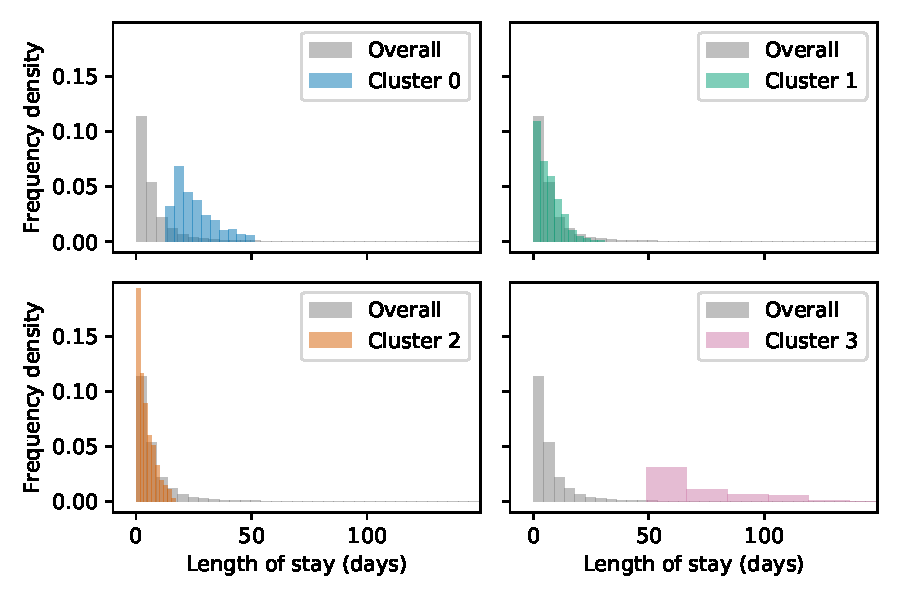
\includegraphics[width=\linewidth]{cluster_los}
        \caption{}\label{fig:cluster_los}
    \end{subfigure}\hfill%
    \begin{subfigure}{\halfimgwidth}
        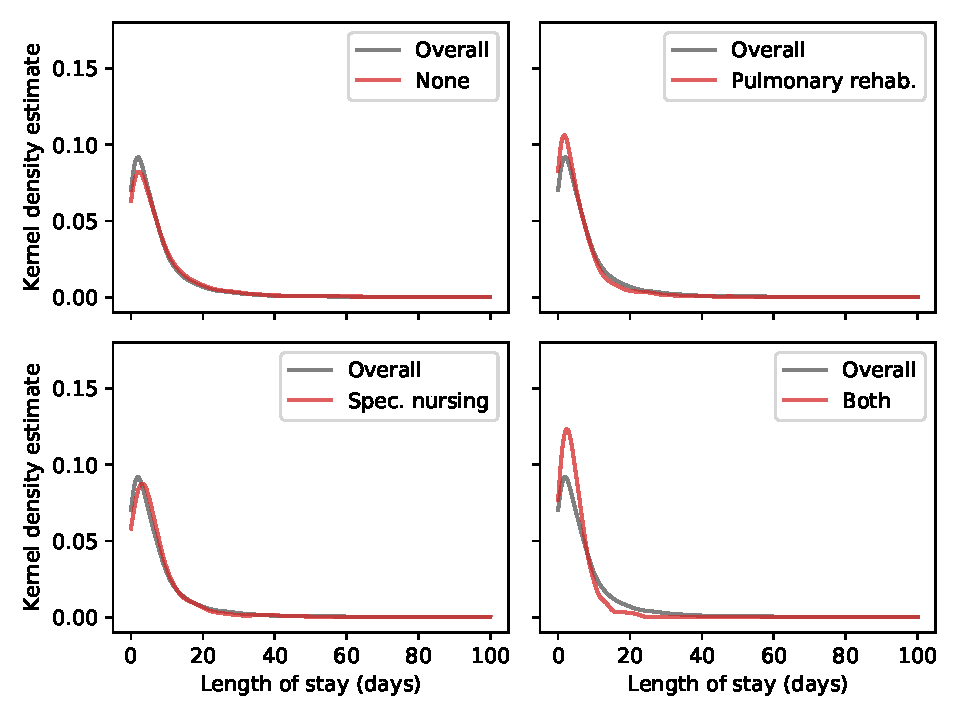
\includegraphics[width=\linewidth]{intervention_los}
        \caption{}\label{fig:intervention_los}
    \end{subfigure}
    \caption{%
        Histograms for length of stay by (\subref{fig:cluster_los}) cluster and
        (\subref{fig:intervention_los}) intervention.
    }\label{fig:los_hist}
\end{figure}

\begin{figure}
    \centering
    \begin{subfigure}{\halfimgwidth}
        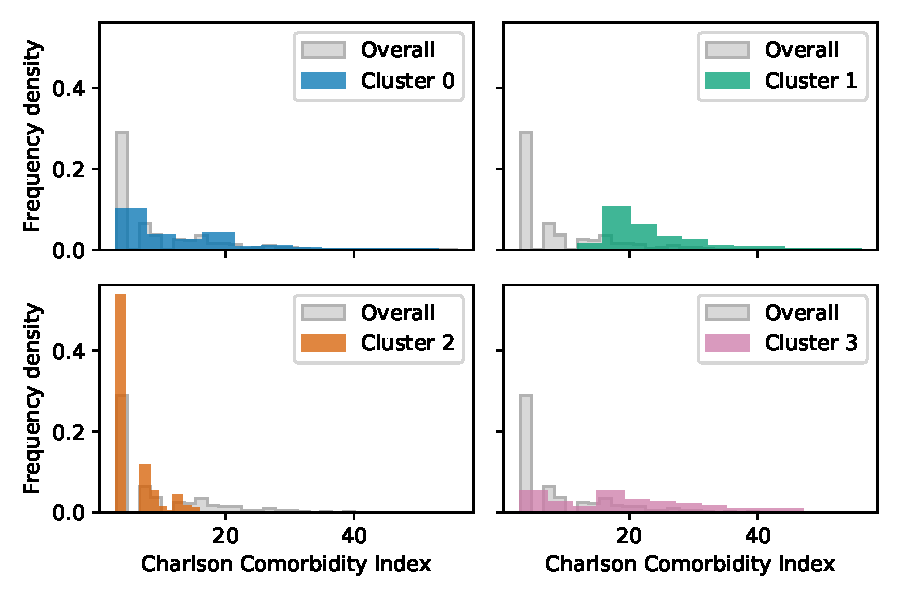
\includegraphics[width=\linewidth]{cluster_charlson_gross}
        \caption{}\label{fig:cluster_charlson}
    \end{subfigure}\hfill%
    \begin{subfigure}{\halfimgwidth}
        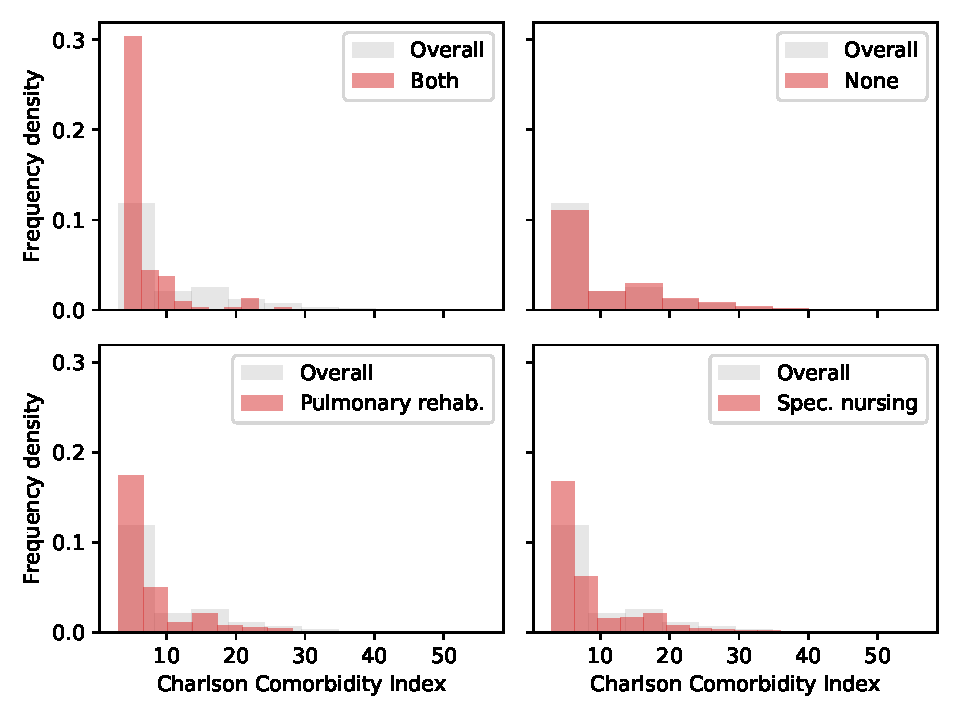
\includegraphics[width=\linewidth]{intervention_charlson_gross}
        \caption{}\label{fig:intervention_charlson}
    \end{subfigure}
    \caption{%
        Histograms for CCI by (\subref{fig:cluster_charlson}) cluster and
        (\subref{fig:intervention_charlson}) intervention.
    }\label{fig:charlson_hist}
\end{figure}

\begin{figure}
    \centering
    \begin{subfigure}{\halfimgwidth}
        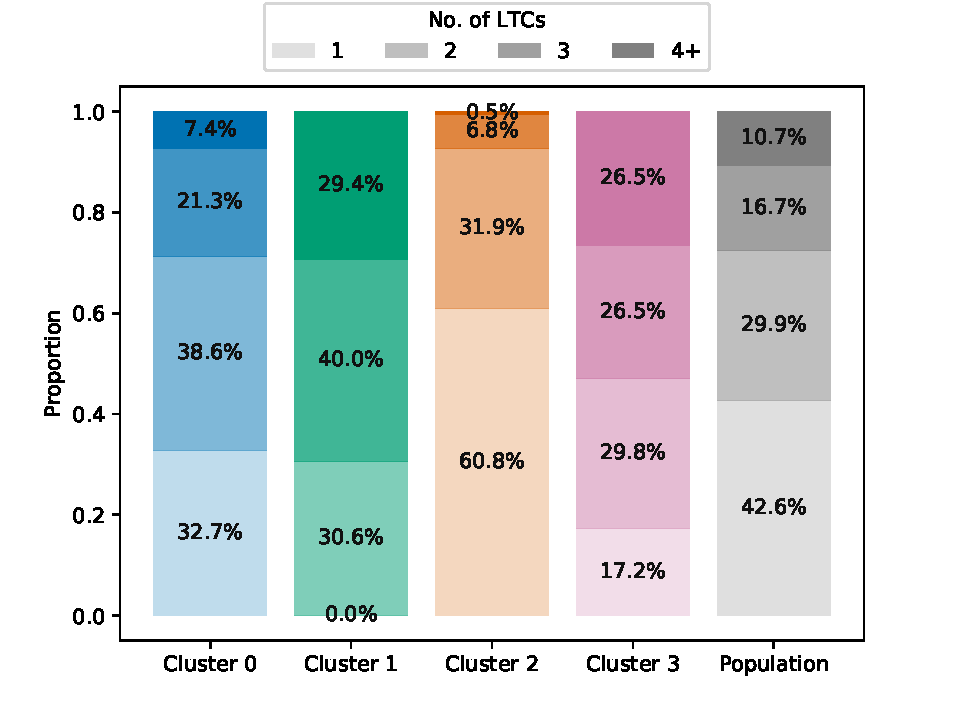
\includegraphics[width=\linewidth]{cluster_ltcs}
        \caption{}\label{fig:cluster_ltcs}
    \end{subfigure}\hfill%
    \begin{subfigure}{\halfimgwidth}
        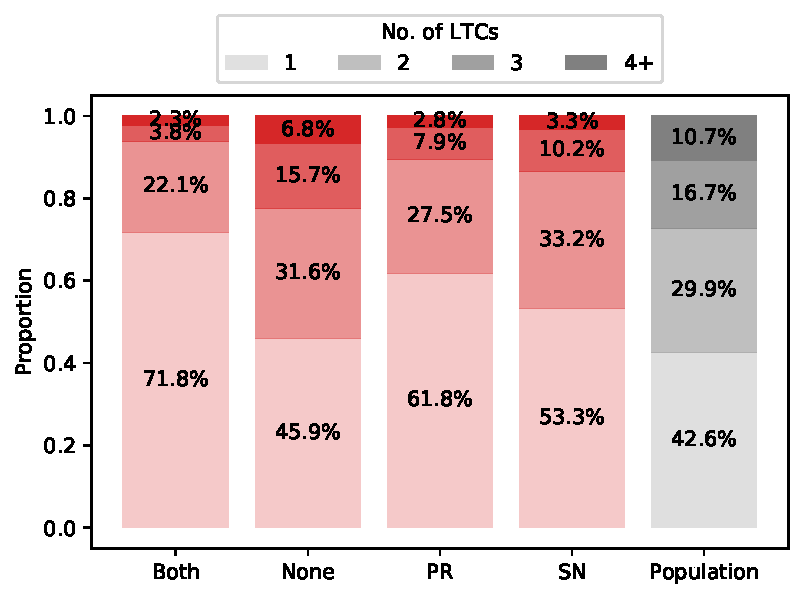
\includegraphics[width=\linewidth]{intervention_ltcs}
        \caption{}\label{fig:intervention_ltcs}
    \end{subfigure}
    \caption{%
        Proportions of concurrent LTC counts presented by patients by
        (\subref{fig:cluster_ltcs}) cluster and (\subref{fig:intervention_ltcs})
        intervention.
    }\label{fig:ltcs}
\end{figure}

\begin{figure}
    \centering
    \begin{subfigure}{\halfimgwidth}
        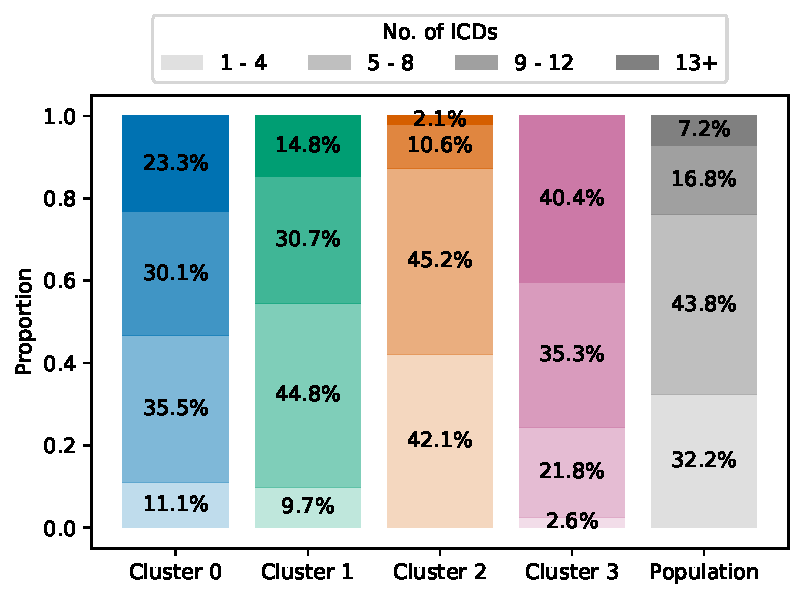
\includegraphics[width=\linewidth]{cluster_icds}
        \caption{}\label{fig:cluster_icds}
    \end{subfigure}\hfill%
    \begin{subfigure}{\halfimgwidth}
        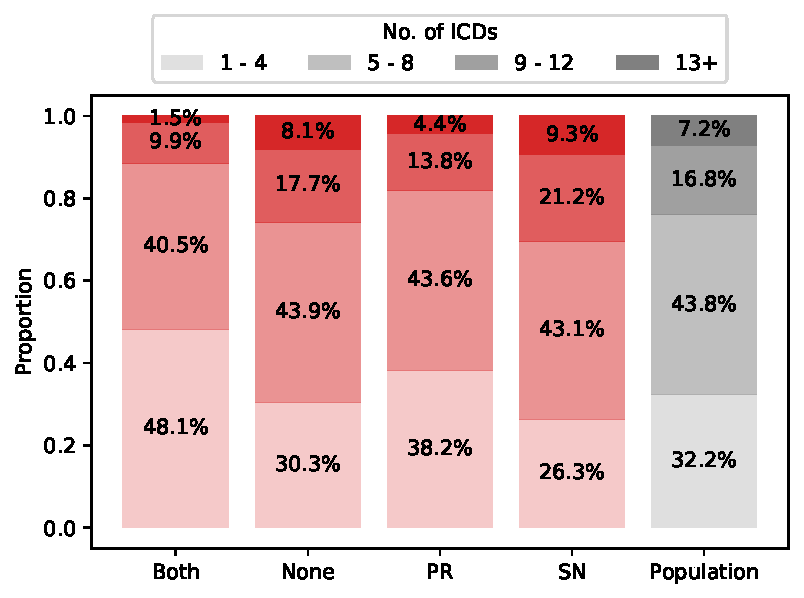
\includegraphics[width=\linewidth]{intervention_icds}
        \caption{}\label{fig:intervention_icds}
    \end{subfigure}
    \caption{%
        Histograms for number of ICDs by (\subref{fig:cluster_icds}) cluster
        and (\subref{fig:intervention_icds}) intervention.
    }\label{fig:icds}
\end{figure}
